
%%%%%%%%%%%%%%%%%%%%%%%%%%%%%%%%%%%%%%%%%%%%%%%%%%%%%%%%%%%
\section{Block-pushing results}\label{sec:expResults}
%%%%%%%%%%%%%%%%%%%%%%%%%%%%%%%%%%%%%%%%%%%%%%%%%%%%%%%%%%%

This section analyzes a \emph{block-pushing} task attempted by both our hybrid, hysteresis-based controller and by human users.  

\subsection{Human-controlled block-pushing}

In previous work over 1000 human users completed an online version of this task using varying levels of feedback.
 The original experiment explored manipulation with varying amounts of sensing information: {\bf full-state} sensing showed the position of all robots; {\bf convex-hull} drew a convex hull around the outermost robots; {\bf mean} displayed the average position of the population; and {\bf mean + variance} added a confidence ellipse. Fig.~\ref{fig:Visualization} shows screenshots of the same robot swarm with each type of visual feedback. Full-state requires $2n$ data points for $n$ robots. Convex-hull requires at worst $2n$, but usually a smaller number.  Mean requires two, and variance three, data points.  Mean and mean + variance are convenient even with millions of robots. We hypothesized a steady decay in performance as the amount of visual feedback decreased.

\begin{figure}[b!]
\renewcommand{\figwid}{0.24\columnwidth}
\begin{overpic}[width =\figwid]{VaryVisFS.pdf}\put(20,15){Full-state}\end{overpic}
\begin{overpic}[width =\figwid]{VaryVisCH.pdf}\put(10,15){Convex-hull}\end{overpic}
\begin{overpic}[width =\figwid]{VaryVisMV.pdf}\put(10,15){Mean + var}\end{overpic}
\begin{overpic}[width =\figwid]{VaryVisMe.pdf}\put(30,15){Mean}\end{overpic}
\caption{\label{fig:Visualization}Screenshots from a block-pushing task with human users. This experiment challenged players to quickly steer 100 robots (blue discs) to push an object (green hexagon) into a goal region. 
%\vspace{-1em}
}
\end{figure}

\begin{figure}
\centering
\begin{overpic}[width = \columnwidth]{ResVaryVis.pdf}\end{overpic}
\vspace{-2em}
\caption{\label{fig:ResVaryVis} Completion-time results for the four levels of visual feedback shown in Fig.~\ref{fig:Visualization}. 
%\vspace{-2em}
}
\end{figure}



To our surprise, the results indicated the opposite: players with just the mean completed the task faster than those with full-state feedback.  As Fig.~\ref{fig:ResVaryVis} shows, the levels of feedback arranged by increasing completion time are [mean, mean + variance, full-state, convex-hull].  Interviews with  beta-testers suggests that tracking 100 robots was overwhelming---similar to schooling phenomenons that confuse predators---while working with just the mean + variance was like using a ``spongy'' manipulator. Convex-hull feedback was confusing and irritating because a single robot left behind an obstacle would distort the entire hull, obscuring the information about the majority of the swarm.
%obscuring what the rest of the swarm is doing.   


\subsection{Automated block-pushing}
Fig.~\ref{fig:story} shows snapshots during an execution of this algorithm. To solve this block-pushing task, we discretized the environment. On this discretized grid we used breadth-first search to determine $\mathbf{M}$, the shortest distance from any grid cell to the goal, and generated a gradient map $\nabla \mathbf{M}$ toward the goal as shown in Fig.~\ref{fig:BFSGradient}.  The block's center of mass is at $\mathbf{b}$ and has radius $r_b$. 
Three constants are needed, where $k_1>k_2>1$ and $1>k_2>0$. All experiments used $[k_1,k_2,k_3] = [2.5,1.5,0.1]$.
The robots were directed to assemble behind the block at  $\mathbf{b} - k_2 r_b \nabla \mathbf{M}(\mathbf{b})$, then move to  $\mathbf{b} - k_3 r_b \nabla \mathbf{M}(\mathbf{b})$ to push the block toward the goal location. We use the hybrid hysteresis-based controller in Alg.~\ref{alg:MeanVarianceControl}  to track the desired position, while maintaining sufficient robot density to move a block by switching to minimize variance whenever variance exceeds a set limit. The minimize variance control law \eqref{eq:PDcontrolVariance} is slightly modified to choose the nearest corner further from the goal than $\mathbf{b}$ with an obstacle-free straight-line path to $\mathbf{b}$. 
The control algorithm  for block-pushing is listed in Alg.~\ref{alg:BlockPushing}. 
Experimental results are summarized in Fig.~\ref{fig:AutoControlVaryN}.  Although larger populations of robots can apply more force, minimizing the variance requires more time with larger populations and dominates task completion time.

\begin{algorithm}
\caption{Block-pushing controller for a robotic swarm.}\label{alg:BlockPushing}
\begin{algorithmic}[1]
\Require Knowledge of swarm mean $[\bar{x},\bar{y}]$, variance $[\sigma_x^2, \sigma_y^2]$,  moveable block's center of mass $\mathbf{b}$, map of the environment, and the locations of all convex corners $\mathbf{C}$
\Require Robot distribution is unimodal
\Require Obstacle-free, straight-line path from swarm to moveable block
\State Compute $\mathbf{M}$, the distance to goal, with breadth-first search
\State Compute the gradient, $\nabla \mathbf{M}$
\State $\mathbf{C} \gets \mathrm{sort(\mathbf{C})}$ according to $-\mathbf{M}$
\While{$\mathbf{b}$ is not in goal region}
\State $\sigma^2 \gets \max{(\sigma_x,\sigma_y)}$
\If {$\sigma^2 > \sigma_{max}^2$}
\While{$\sigma^2 > \sigma_{min}^2$}
\State $\mathbf{c}_i \gets$ the nearest corner in $\mathbf{C}$ to $[\bar{x},\bar{y}]$
\State $ [x_{goal}, y_{goal}] \gets \mathbf{c}_i $
\If {$\mathbf{M}(\mathbf{b}) > \mathbf{M} (\mathbf{c}_i)$}
\State  $[x_{goal}, y_{goal}] \gets  \mathbf{c}_{i-1}$ 
\State Apply \eqref{eq:PDcontrolPosition} to move toward $[x_{goal}, y_{goal}]$
\EndIf
\EndWhile
\Else  
\If {$\mathrm{distance}( \mathbf{b}, [x_{goal}, y_{goal}] ) > k_1 r_b$}
	\State$r_p \gets k_2 r_b$  \Comment{guarded move}
	\Else
	\State$r_p \gets k_3 r_b$  \Comment{pushing move}
	\EndIf
\State $[x_{goal}, y_{goal}] \gets \mathbf{b} - r_p \nabla \mathbf{M}(\mathbf{b})$ 
\EndIf
\State Apply \eqref{eq:PDcontrolPosition} to move toward $[x_{goal}, y_{goal}]$
\EndWhile
\end{algorithmic}
\end{algorithm}



\begin{figure*}
\centering
\renewcommand{\figwid}{0.3\columnwidth}
\href{http://youtu.be/tCej-9e6-4o}{\begin{overpic}[width =\figwid]{story1.png}\put(6,15){T = 5 s}
\end{overpic}
\begin{overpic}[width =\figwid]{story2.png}\put(6,15){T = 12 s}
\end{overpic}
\begin{overpic}[width =\figwid]{story3.png}\put(6,15){T = 20 s}
\end{overpic}
\begin{overpic}[width =\figwid]{story4.png}\put(6,15){T = 25 s}
\end{overpic}
\begin{overpic}[width =\figwid]{story5.png}\put(6,15){T = 33 s}
\end{overpic}}
\caption{\label{fig:story}\href{http://youtu.be/tCej-9e6-4o}{Snapshots showing the block-pushing experiment with 200 robots under automatic control.}
%\vspace{-2em}
}
\end{figure*}

\begin{figure}
\centering
\begin{overpic}[scale=0.3]{BFSMode.png}
\end{overpic}
\begin{overpic}[scale=0.3]{GradientView.png}
\end{overpic}
\caption{\label{fig:BFSGradient}The BFS algorithm finds the shortest path for the moveable block (left), which is used to compute gradient vectors (right).
%\vspace{-2em}
}
\end{figure}




\begin{figure}
\centering
\begin{overpic}[width = \columnwidth]{AutoControlVaryN.pdf}\end{overpic}
\vspace{-2em}
\caption{\label{fig:AutoControlVaryN} Completion-time results using the automatic controller from Alg.~\ref{alg:BlockPushing} for different numbers of robots.  Each bar is labelled with the number of trials.
}
\end{figure}





Algorithm \ref{alg:BlockPushing} is an imperfect solution and has a failure mode if the robot swarm becomes multi-modal with modes separated by an obstacle, as shown in Fig.~\ref{fig:Failure}.  In this case, moving toward a corner will never reduce the variance below $\sigma_{min}^2$.


  The first challenge is to identify when the distribution has become multi-modal.  Measuring just the mean and variance is insufficient to determine if a distribution is no longer unimodal, but if the swarm is being directed to a corner, and the variance does not reduce below $\sigma_{min}^2$, the swarm has become separated. In this case, we must either manipulate with a partial swarm, or run a gathering algorithm.  For the  `{\sffamily S}'-shaped workspace in this study, an open-loop input that commands the swarm to move in succession \{{\sc left, down, right, down}\} will move the swarm to the bottom right corner.
This is not true for all obstacle fields. In a  `{\sffamily T}'-shaped workspace, it is not possible to find an open-loop input that will move the entire swarm to the bottom of the `{\sffamily T}'.  
 
  Using only the mean and variance may be overly restrictive.  Many heuristics using high-order moments have been developed to test if a distribution is multimodal~\cite{haldane1951simple}.  Often the sensor data itself, though it may not resolve individual robots, will indicate multi-modality.  For instance CCD images reveal clusters of bacteria, and MRI scans show agglomerations of particles~\cite{stuber2007positive}.  This data can be fitted with $k$-means or expectation maximization algorithms, and manipulation could be performed with the nearest swarm of sufficient size.
  

\begin{figure}
\centering
\begin{overpic}[scale=0.3]{FailureBlockPush.png}
\end{overpic}
\begin{overpic}[scale=0.3]{FailureBlockPushing}
\end{overpic}
\caption{Algorithm \ref{alg:BlockPushing} fails when some robots are separated by the maze and the swarm can not achieve $\sigma^2 < \sigma_{min}^2$.  These failures occured during 14\% of trials.\label{fig:Failure}
%\vspace{-2em}
}
\end{figure}


\subsection{Hardware system}


Our experiments are on centimeter-scale hardware systems called \emph{kilobots}.  These allows us to emulate a variety of dynamics, while enabling a high degree of control over robot function, the environment, and data collection. The kilobot \cite{Rubenstein2012,rubenstein2014programmable} is a low-cost robot designed for testing collective algorithms with large numbers of robots. It is available commercially or as an open source platform~\cite{K-Team2015}.  Each robot is approximately 3 cm in diameter, 3 cm tall, and uses two vibration motors to move on a flat surface at speeds up to 1 cm/s.  Each robot has one ambient light sensor that is used to implement \emph{phototaxis},  moving towards a light source. 
In these experiments as shown in Fig.~\ref{fig:setup}, we used $n$=64 kilobots, a 1.5 m$\times$1.2 m whiteboard as the workspace, and four 30W LED floodlights arranged 1.5 m above the plane of the table at the $\{N,E,S,W\}$ vertices of a 6 m square centered on the workspace. The lights were controlled using an Arduino Uno board connected to an 8 relay shield board.  At top of the table, an overhead machine vision system was added to track the position of the swarm. Laser-cut patterns for our neon green fiducial markers and our {\sc Matlab} tracking code are available at our github repository~\cite{Shahrokhi2015GitHubShapeControl}.


\begin{figure}
\begin{center}
	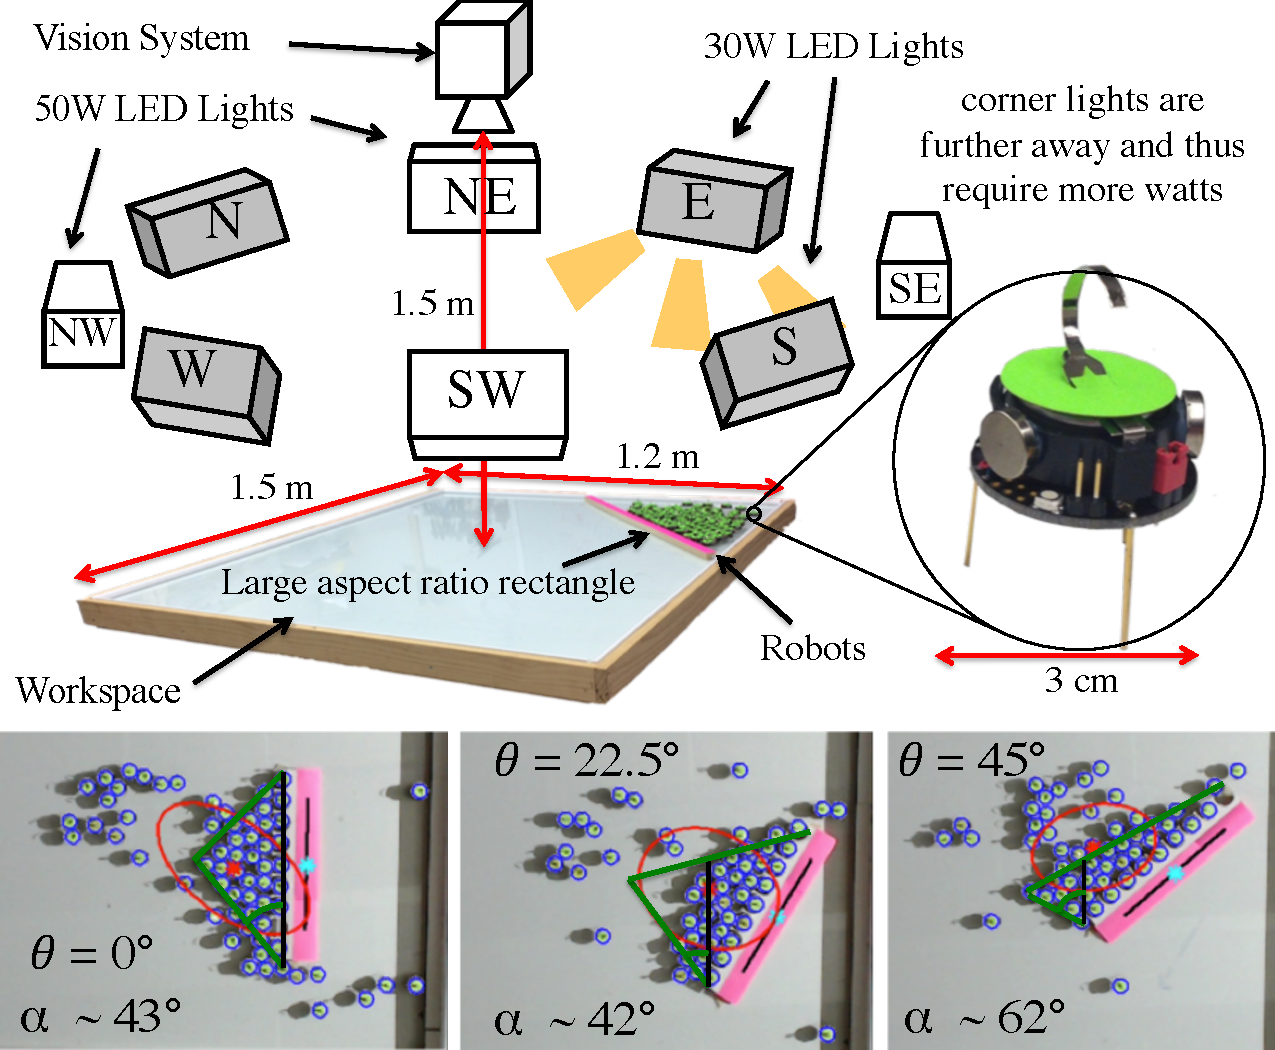
\includegraphics[width=\columnwidth]{SetUp.pdf}
\end{center}
\caption{\label{fig:setup}
Hardware platform:  table with 1.5$\times$1.2 m workspace, surrounded by eight remotely triggered 30W LED floodlights, with an overhead machine vision system.
}
\end{figure}

The walls of the hardware platform have almost infinite friction, due to the three legged design of the kilobots. When a kilobot is steered into the wall, they pin themselves to the wall until the light changes direction and they begin turning in the other direction.  This wall friction is sufficient to enable independent position control of two kilobots, as shown in Fig.~\ref{fig:storyReal}.



\begin{figure*}
\centering
\renewcommand{\figwid}{0.3\columnwidth}
{
\begin{overpic}[width =0.315\columnwidth]{twoR_1.pdf}\put(15,65){$t$  = 30 s}\end{overpic}\hspace{-.5em}
\begin{overpic}[width =\figwid]{twoR_2.jpg}\put(15,65){$t$  = 60 s}
\end{overpic}
\begin{overpic}[width =\figwid]{twoR_3.jpg}\put(15,65){$t$  = 90 s}
\end{overpic}\\
\vspace{1em}
\begin{overpic}[width =\figwid]{twoR_4.jpg}\put(15,65){$t$  = 120 s}
\end{overpic}
\begin{overpic}[width =\figwid]{twoR_5.jpg}\put(15,65){$t$  = 150 s}
\end{overpic}}
\caption{\label{fig:storyReal}{Two robot positioning using the hardware setup and two kilobot robots.  The walls have nearly infinite friction, as illustrated by this fig, the robot with the blue path that is stopped by the wall until the light changes orientation, while the orange robot in free-space is unhindered.}
%\vspace{-2em}
}
\end{figure*}



To demonstrate covariance control $n=64$ robots were placed on the workspace and manually steered with a single light source, using friction with the boundary walls to vary the covariance from  -5000 to 10,000.  The resulting covariance is plotted in Fig.~\ref{fig:covExperiment}, along with snapshots of the swarm.




\begin{figure}
\begin{center}
	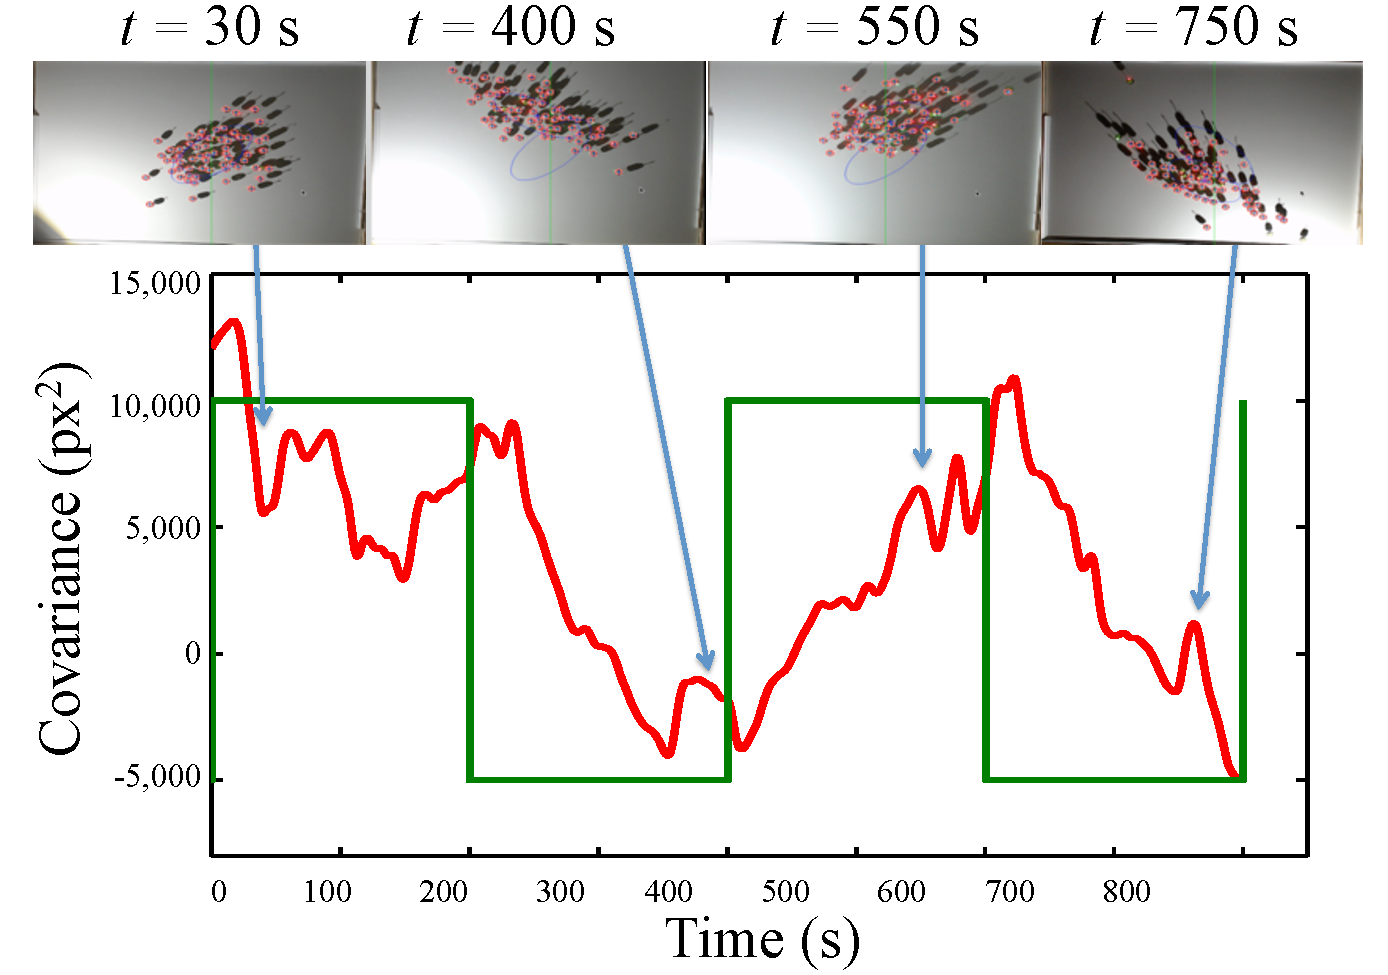
\includegraphics[width=\columnwidth]{experiment.pdf}
\end{center}
\caption{\label{fig:covExperiment}Hardware demonstration steering 64 kilobot robots to desired covariance.  Frames above the plot show output from machine vision system and an overlaid covariance ellipse.
}
\end{figure}




